\chapter{Literature Review}
\label{cha:literature-review}

\section{Measuring complexity}

\section{Emergence}
The notion of emergence is central to the study of complex systems. It is a very
broad concepts that could be phrased as \emph{the properties an composite entity
  acquires that its composing parts did not have}. Emergence is often described
as being similar to self-organization. Although these two concepts are closely
related, they are fundamentally different ideas
\parencite{dewolfEmergenceSelfOrganisationDifferent2005}. Both properties can
exist independently within a dynamical system.

There seems to be qualitatively different kinds of emergence, which
\cite{dehaanHowEmergenceArises2006} describe as Discovery, Mechanistic
emergence, and Reflective emergence. These correspond to different levels, or
``strengths'' of emergence, from fractal patterns to complex social systems and
ecosystems.

A subset of research on emergence has focused on complex adaptive systems. In
such systems, emergence is explicitly used to refer to macro-level patterns
arising from interacting agents \parencite{hollandEmergenceChaosOrder2000,
  kauffmanHomeUniverseSearch1995, langtonStudyingArtificialLife1986}.


\section{Evolutionary algorithms}
Evolutionary algorithms are the class of algorithms inspired by natural
biological processes, in particular evolution. There a many types of
evolutionary algorithms, from genetic algorithms to quality diversity and
novelty search \parencite{lehmanAbandoningObjectivesEvolution2011,
  lehmanEvolvingDiversityVirtual2011}.

\subsection{Novelty search}
The idea behind \ac{NS} is to drive a search algorithm by the novelty of
produced behavior \parencite{lehmanAbandoningObjectivesEvolution2011}. The most
surprising feature of this algorithm is that the actual objective of the task is
not taken into account at all during the search process. Generated agents are
evaluated solely on the novelty of their behavior. Despite this, it appears to
be at least as efficient as other search processes that are goal focused, such
as maze navigation and biped locomotion
\parencite{lehmanAbandoningObjectivesEvolution2011}, swarm robotics
\parencite{gomesEvolutionSwarmRobotics2013}, or neural network design
\parencite{risiEvolvingPlasticNeural2010}.

This method has some limits, which are caused by a relative lack of theoretical
understanding of the effects of the parameters of \ac{NS}. The choice of
behavior descriptors for determining the novelty of agents is also not
straightforward. Several empirical studies have investigated the impact of a
range of parameters on the performance of \ac{NS}
\parencite{gomesDevisingEffectiveNovelty2015,
  kistemakerCriticalFactorsPerformance2011}, while other works have begun to
shed light on the theory \parencite{doncieuxNoveltySearchTheoretical2019}. In
practice \ac{NS} algorithms are expected to cover the exploration space well
\parencite{cullyQualityDiversityOptimization2017,pughQualityDiversityNew2016},
in some cases uniformly \parencite{gomesDevisingEffectiveNovelty2015}. \ac{NS}
algorithms are related to genetic algorithm since they maintain a population,
that is a set of individuals used to measure the novelty of current solutions.
There is also an archive of behavior of previous individuals to ensure that the
novelty is measured against all previously generated behaviors. There exists
multiple strategies for maintaining this archive
\parencite{gomesDevisingEffectiveNovelty2015}. Some use individuals whose
novelty was above a threshold when first evaluated
\parencite{lehmanAbandoningObjectivesEvolution2011}, the most novel individuals
of each generation \parencite{liapisConstrainedNoveltySearch2015}, random
individuals from the past generations
\parencite{lehmanEfficientlyEvolvingPrograms2010}, or none at all
\parencite{mouretEncouragingBehavioralDiversity2012}.

The principle of guiding search by novelty alone is closely related to this
thesis, especially with the challenge of parametrizing and searching the space
of available complex systems without using any explicit goal function. The goal
of \ac{NS} is to carry out search without a goal function, and we draw
inspiration from this algorithm.

\section{Open-ended evolution}
The field of Artificial Life research has worked to figure out what the
fundamental conditions for the emergence of living systems are, and how to
create a process that can display analogous levels of creativity and complexity
as natural evolution \parencite{eigenHypercycle1979,
  langtonArtificialLifeProceedings1989, dysonOriginsLife1999,
  stanleyWhyOpenEndednessMatters2019, packardOverviewOpenEndedEvolution2019,
  sorosOpenendednessLastGrand2017}. It build upon the data and understanding we
collected about the process of life, but abstracts from any specific living
process and attempts to integrate various approaches into one unified research
to extract the first principles of life. A major assumption underpinning this
research is that this natural evolution as a process can be implemented equally
well in different media \parencite{dennettDarwinDangerousIdea1996}.

A system that behaves like natural evolution, producing a seemingly endless
amount of novelty and complexity starting from elementary building blocks is
called \emph{open-ended}. The main challenge of \ac{OEE} is there is not a simple
single test for the phenomenon, but instead there are different kinds of
open-ended evolution. Systems can exhibit more than one kind at a time. In the
report from a workshop on \ac{OEE} at York
\parencite{taylorOpenEndedEvolutionPerspectives2016}, the authors summarized the
different kinds of \ac{OEE}, which were further refined in a follow up work
\parencite{packardOverviewOpenEndedEvolution2019}. They are as follows

\begin{enumerate}
  \item Interesting new kinds of entities and interactions
  \item Evolution of evolvability
  \item Major transitions
  \item Semantic evolution
\end{enumerate}

The first category describes the ability of a system to construct new entities
with different properties, behavior, or interactions with other entities. For
example, the Tierra simulation sees entities emerge that exploit the computing
power of others, acting as parasites \parencite{srayApproachSynthesisLife1991}.
The second type is related to how open-end evolution itself can be evolved
through the emergence of multiple ``stepping stones'' that enable higher level
evolutionary units to be used by individuals or through interactions
\parencite{patteeEvolvedOpenEndednessNot2019}.

\subsection{Defining open-endedness}

Several necessary conditions and requirements have been identified across the
\ac{OEE} literature, which form an overlapping set of potential research
directions for developing open-ended systems. We list a few of these conditions
here. First, \cite{maleyFourStepsOpenended1999} identifies four requirements:

\begin{enumerate}
  \item An open-ended evolutionary system must demonstrate unbounded diversity
        during its growth phase.
  \item An open-ended evolutionary system must embody selection.
  \item An open-ended evolutionary system must exhibit continuing new adaptive
        activity.
  \item An open-ended evolutionary system must have an endogenous implementation
        of niches.
\end{enumerate}
Next, \cite{sorosIdentifyingNecessaryConditions2014} identified four more necessary
conditions which are as follows

\begin{enumerate}
  \item A rule should be enforced that individuals must meet some minimal
        criterion (MC) before they can reproduce, and that criterion must be
        nontrivial.
  \item The evolution of new individuals should create novel opportunities for
        satisfying the MC.
  \item Decisions about how and where individuals interact with the world should
        be made by the individuals themselves.
  \item The potential size and complexity of the individuals' phenotypes should
        be (in principle) unbounded.
\end{enumerate}
Then, \cite{taylorRequirementsOpenEndedEvolution2015} also stated five
requirements for an open-ended system:

\begin{enumerate}
  \item Robustly reproductive individuals.
  \item A medium allowing the possible existence of a practically unlimited
        diversity of individuals and interactions, at various levels of
        complexity.
  \item Individuals capable of producing more complex offspring.
  \item An evolutionary search space that typically offers mutational pathways
        from one viable individual to other viable (and potentially fitter )
        individuals.
  \item Drive for continued evolution.
\end{enumerate}
Taylor also states a more general condition that should be sufficient for
creating an open-ended system as ``evolutionary dynamics in which new,
surprising, and sometimes more complex organisms continue to appear''
\parencite{taylorRequirementsOpenEndedEvolution2015,
  taylorOpenEndedEvolutionPerspectives2016}.

All these conditions illustrate a major challenge of \ac{OEE} research: the lack
of clear definition or notion of what conditions make a system open-ended. We
seem to agree about what is not open-ended, but whenever a constraint or
requirement for \ac{OEE} is identified, subsequent evidence forces us to refine
them later. This is related to the problem of complexity, for which no single
definition exists \parencite{johnsonSimplyComplexityClear2009}.

A common process to produce systems that behave analogously to natural evolution
is to start from evolvable units or building blocks
\parencite{srayApproachSynthesisLife1991, simsEvolvingVirtualCreatures1994,
  ofriaAvidaSoftwarePlatform2004, yaegerComputationalGeneticsPhysiology1994,
  channonImprovingStillPassing2003, spectorDivisionBlocksOpenended2007,
  sorosIdentifyingNecessaryConditions2014}. The reason is that starting from
higher level primitive units whose emergence would be hard to characterize may
be easier and faster than starting from lower level components. Results obtained
from these systems are often surprising, since they bear some key resemblance to
natural evolutionary processes. For example we note the emergence of parasitic
entities within the Tierra simulation \parencite{srayApproachSynthesisLife1991}.
The process of emergence of these building blocks from simple rules and
components has also been investigated significantly
\parencite{bagleySpontaneousEmergenceMetabolism1991,
  huttonEvolvableSelfReproducingCells2007, flammEvolutionMetabolicNetworks2010,
  sayamaSeekingOpenendedEvolution2011}. It appears harder to bridge the gap and
create high level evolutionary-like processes and behaviors from elementary
rules and substrates.

\subsection{Open-endedness in cellular automata}
One class of system that has rich interactions between each of its components as
well as no predefined evolvable units or assumptions about individuality is the
\ac{CA}. One of the very first automata, Von Neumann's self-reproducing machine,
was designed with goals that align with open-ended evolution, which is to build
a machine with no central controller and limited local interaction that can
self-reproduce as a whole
\parencite{vonneumannTheorySelfreproducingAutomata1966,
  pesaventoImplementationNeumannSelfReproducing1995}. Later, other
self-replicating structures such as Langton's loop
\parencite{langtonSelfreproductionCellularAutomata1984} and evoloops
\parencite{sayamaNewStructurallyDissolvable1999,
  salzbergComplexGeneticEvolution2004} showed that more properties of open-ended
systems can be included in a \ac{CA}. An potential limitation of \acp{CA} is the
absence of notion of conservation of ``matter''. For example, the game of life
can start from a configuration with very few live cells and create many more at
no cost during its evolution. Some authors believe that this conservation
property is essential to the construction of an open-ended evolving system
\parencite{taylorChapterCreativityEvolution2002}.

\subsection{Artificial chemistries}
Most of the time, \acp{AC} are not trying to accurately model chemical processes
(as in \parencite{ostrovskyCellularAutomataPolymer2001} for example). Instead,
they build models of the dynamics of complex molecular processes that lead to
evolutionary behavior \parencite{dittrichArtificialChemistriesReview2001}. By
abstracting away from the natural molecular processes, \acp{AC} tries to uncover
fundamental conditions for the emergence of organization, self-maintenance, or
self-construction with basic building blocks. There are various approaches for
building these \aclp{AC}, of which we review a few here.

\paragraph{Rewriting systems.}
Rewriting systems are composed of entities or symbols that get modified
according to a set of syntactic rules. Patterns of symbols or entities are
replaced according to these rules.

\paragraph{Cellular automata.}
\Acfp{CA} can be see as a particular case of lattice molecular systems. For
example the autopoietic system introduced by
\cite{varelaAutopoiesisOrganizationLiving1991} is a 2d square grid with sites
that be occupied by \emph{atoms} which is similar to a \ac{CA} with 4 states.
Each of these states is analogous to a chemical component of the system: ($\emptyset$)
empty site, (S) substrate, (K) catalyst and (L) monomer. Basic rules are applied
asynchronously and define how neighboring atoms interact with each other.
Remarkably, stable self-repairing cells arise spontaneously from these basic
rules. Their membrane is composed of a chain of monomers, which is maintained by
the substrate and catalyst reacting according to the rules. Some key components
were investigated in other works, showing that they are crucial for autopoeisis
to be possible \parencite{zelenySelforganizationLivingSystems1977,
  mcmullinRediscoveringComputationalAutopoiesis1997}.

\section{Computing with complex systems}

The problem of computing within complex systems is closely related to the
question of decentralized parallel computation in general, for which there exist
an abundant literature. Different paradigms exist for controlling and harvesting
the computations within complex systems. Several other names have been used for
closely related topics, such as organic computing
\parencite{muller-schloerOrganicComputingParadigm2011} which is the study of
systems with life-like properties such as self-organization or the ability to
adapt to a dynamically changing environment. Agent-based computing
\parencite{jenningsAgentBasedComputingPromise1999} focuses on computing systems
composed of several autonomous agents. Amorphous computing
\parencite{abelsonAmorphousComputing2000,
  nagpalProgrammablePatternFormationScaleIndependence2008,
  nagpalProgrammableSelfassemblyUsing2002} is about making vast quantities of
individual computing elements work, and to ensure ``the cooperation of vast
numbers of unreliable parts interconnected in unknown, irregular, and
time-varying ways''.

\subsection{Computing in cellular automata}

\Acfp{CA} are decentralized parallel systems with many identical components with
local connectivity. Because of these properties, they have the potential to
carry out robust, efficient computations. \ac{CA}-based computing machines could
recover from perturbations or carry out computations in stochastic environments.
Moreover, they are also interesting for modeling the behavior of natural complex
systems. For more details about \acp{CA}, see section
\ref{sec:cellular-automata-sec}.

\paragraph{Von Neumann's self-reproducing \ac{CA}}

\paragraph{Universal Computation in Cellular Automata}
It is not difficult to see that a \ac{CA} can be capable of universal
computation. The basic approach is to show that it can simulate a Turing
machine, which we assume has an infinite tape. A \ac{CA} rule can be constructed
by reproducing all the steps of a Turing machine's behavior while adding a state
to each cell indicating wether it is active or not, and enforcing that only one
cell is active at a time. This turns the parallel \ac{CA} into a sequential
object that simulates a Turing machine. A similar construction was carried out
by \parencite{smithSimpleComputationUniversalCellular1971}, making a \ac{CA}
with one-to-one correspondence between its time steps and that of a target
Turing machine.

\paragraph{Evolving \acp{CA} with genetic algorithms}
A major step forward from the clever but difficult hand-design of \acp{CA} rules
to perform computations is the use of learning algorithms to automatically
design those rules \parencite{mitchellEvolvingCellularAutomata1996}.

Genetic algorithms are a type of search method inspired by biological evolution
\parencite{bookerClassifierSystemsGenetic1989}. Candidate solutions to a problem
are encoded as \emph{chromosomes}, that is a structured data representation that
can be modified incrementally. In practice it is often chosen to be a string of
bits.

\paragraph{Reliable computation in cellular automata}
The problem of carrying out reliable computations in \acp{CA} is studied early
on in its history because of the potential of that model for real hardware
implementation. The first studies used probabilistic approaches for solving the
error detection and correction problems of automata --- which includes other
models than \acp{CA} \parencite{neumannProbabilisticLogicsSynthesis1956,
  winogradReliableComputationPresence1963,
  ,tsertsvadzeStochasticAutomataProblem1964,
  ,haraoConsiderationCellularAutomata1973}. Other methods make use of the
special structure of \ac{CA}, but rely on strong assumptions about the
likelihood of errors \parencite{haraoFaultTolerantCellular1975,
  nishioFaultTolerantCellular1975}. Peter Gács has shown how to construct a 1-d
CA which can perform arbitrarily large reliable computations, with each cell an
error with a positive probability
\parencite{gacsReliableComputationCellular1986}. The fault model he describes is
important from the point of view of ergodic theory because Gács’ result
invalidates the ``positive probability conjecture'' in statistical physics,
which states that all one dimensional infinite particle system with positive
transition probabilities is ergodic. For more recent work on fault-tolerance by
Gács, see \parencite{gacsReliableCellularAutomata2001}.

\paragraph{Neural cellular automata}
The principle of \ac{NCA} is based on the analogy between \acp{CA} and two types
of neural networks: \acp{RNN} and \acp{CNN} (see Section
\ref{sec:cell-autom-rnns} for more details about the analogy). Once this link is
established, \ac{NCA} can be manipulated like neural networks, using automatic
differentiation, backpropagation and optimization algorithms to make these
models learn some target task. A first example used this neural network
representation to learn a \ac{NCA} version of existing \ac{CA} rules from
recorded examples of their evolution
\parencite{gilpinCellularAutomataConvolutional2018}. The structure of the
training process and final error of the resulting model is used by the author as
a tool to understand the complexity and properties of the original \ac{CA}.

\acp{NCA} were also used to learn to produce stable self-repairing patterns that
resemble a target image \parencite{mordvintsevGrowingNeuralCellular2020}. The
training process is structured in such a way that the \ac{NCA} needs to learn to
maintain the pattern stable across time and space, but also recover form random
perturbations that are introduced randomly. This results in an interesting demo,
where a pattern is generated and maintained in real time by a \ac{NCA} while a
user can directly apply
perturbations\footnote{\url{https://distill.pub/2020/growing-ca/}}.

\begin{figure}[htbp]
  \centering
  \begin{subfigure}[t]{.49\linewidth}
    \centering
    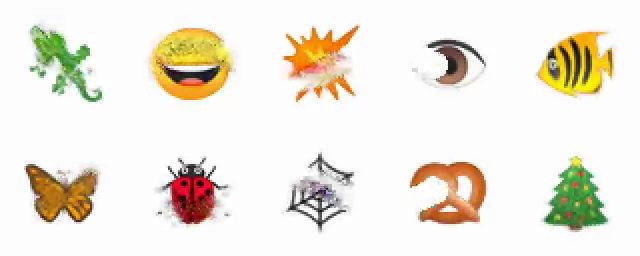
\includegraphics[width=\linewidth]{figures/nca_perturb.png}
    \caption{Perturbed patterns}
    \label{fig:nca_perturb}
  \end{subfigure}
  \begin{subfigure}[t]{.49\linewidth}
    \centering
    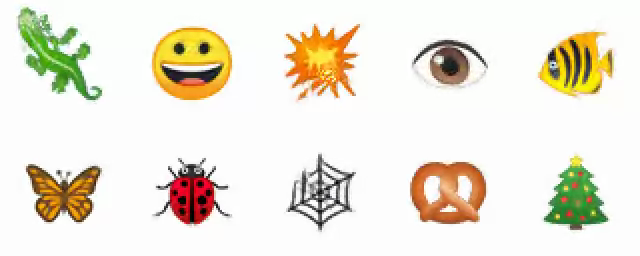
\includegraphics[width=\linewidth]{figures/nca_recover.png}
    \caption{Recovered patterns after a few hundred \ac{NCA} steps.}
    \label{fig:nca_recover}
  \end{subfigure}
  \caption[Resistance of patterns]{Resistance of patterns to perturbations with
    \acp{NCA}. \ac{NCA} can robustly maintain patterns, even under relatively
    strong perturbations (~10-20\% of the pattern's size). This image was
    generated with an online notebook based on code from Alexander
    Mordvintsev\footnotemark.}
  \label{fig:nca}
\end{figure}
\footnotetext{\url{https://colab.research.google.com/github/google-research/self-organising-systems/blob/master/notebooks/growing_ca.ipynb}}

The same authors also used \ac{NCA} to learn to classify digits from the MNIST
database of handwritten digits
\parencite{randazzoSelfclassifyingMNISTDigits2020}. The particularity of this
model is its ability to perform the classification in a decentralized way, by
having the \ac{NCA} change the color of the digits directly in the \ac{CA} grid.
Cells can only communicate with their direct neighbors, so the model has to
reach a consensus by propagating information across the grid. This is done in
parallel, so multiple digits can be classified simultaneously through this
progressive consensus
process\footnote{\url{https://distill.pub/2020/selforg/mnist/}}.
Another work used the same model to learn to continuously generate images with
the same texture as a target \parencite{niklassonSelfOrganisingTextures2021}.
Again, an advantage of this method is the ability to recover from perturbations.

\begin{figure}[htbp]
  \centering
  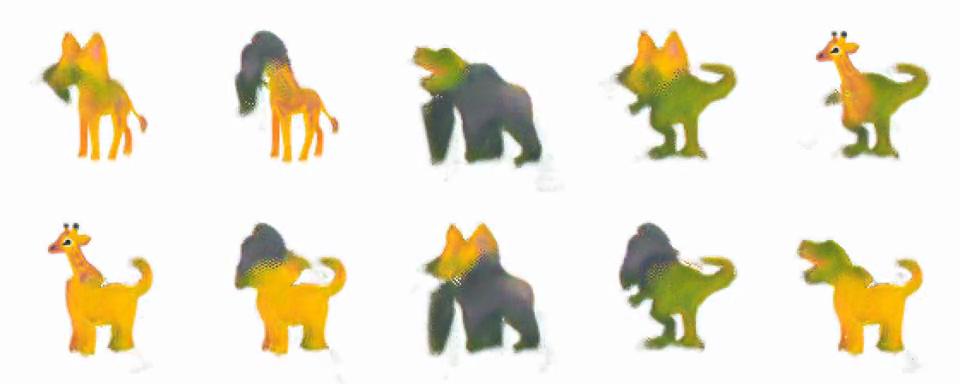
\includegraphics[width=.8\linewidth]{figures/nca_hybrids.png}
  \caption{Examples of stable hybrids obtained with \acp{NCA} trained with the
    method of \parencite{cisnerosOpenendedCreationHybrid2021}.}
  \label{fig:nca_hybrid}
\end{figure}


We used \ac{NCA} as part of our submission to the Minecraft open-endedness
challenge 2021\footnote{\url{https://evocraft.life/}}, a competition organized
at the Gecco 2021 conference competition
track\footnote{\url{https://gecco-2021.sigevo.org/Competitions}}
\parencite{cisnerosOpenendedCreationHybrid2021}. The goal was to build an
open-ended system within the computer game Minecraft. This means building a
systems that fullfils the following requirements:

\begin{itemize}
  \item Divergence: Open-ended algorithms are not expected to slow down or
        converge but rather keep expanding and generating more complex outputs
        over time.

  \item Diversity: Does the algorithm produce entities with strong phenotypic
        diversity?

  \item Complexity: Can the algorithm produce complex entities or entities
        interactions that give rise to complex systems? Are hierarchical and
        modular structures present?

  \item Ecological interactions: Do the created entities interact with each
        other?

  \item Life-Like properties: Inspiration may be taken from other attributes of
        living systems.
\end{itemize}

In each of the examples in figure \ref{fig:nca}, a separate \ac{CA} was trained
on a pattern starting from a single black pixel. We extend this by training a
single \ac{NCA} on multiple patterns from different seeds. Instead of a single
black cell, a small number of black cells are arranged into simple shapes We
call these patterns \emph{seeds}. \ac{NCA} have a lot of parameters. This
allowed us to learn more than one pattern (or larger patterns) without adding
parameters in the architecture. The resulting patterns are of slightly lower
quality but still stable under perturbations and able to grow.

We turned the process of combining seed patterns into a “game” by allowing user
interaction with the evolving CA through Minecraft. Our system is not open-ended
by itself, but needs human interaction to play with the shapes and seed
patterns. This is in the spirit of open-ended games like Picbreeder
\parencite{secretanPicbreederCaseStudy2011, woolleyDeleteriousEffectsPriori2011}
where players choose which generated patterns to mutate or evolve from. The
algorithms can generate endless novelty but human interactions provide the
missing step to make it open-ended.

\subsection{Amorphous computing}
The goal of amorphous computing is to study and define the problem of computing
with multiple interconnected components that are unreliable, irregular,
time-varying and with limited computational capacity
\parencite{abelsonAmorphousComputing2000}. The motivation for this research is
the development of biological substrates that can compute, function as sensors
and actuators, and robustly self-organize to compute with little cost. Precise
manufacturing of chemical or biological substrate with the ability to
communicate locally through chemical or physical interactions is within reach,
making the perspective of using them as computing vessels particularly
attractive. We can embed millions of chips with sensors
\parencite{abelsonAmorphousComputing2000} or program biological cells to serve
as logic gates \parencite{weissProgrammingBiologicalCells1998,
  weissVivoDigitalCircuits2002} while relying on cheaper, decentralized parts
\parencite{buteraProgrammingPaintableComputer2002}.

\begin{figure}[htbp]
  \centering
  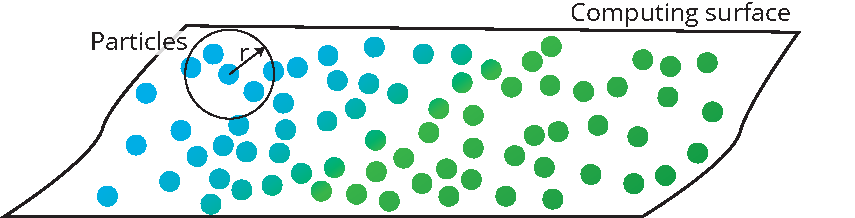
\includegraphics[width=.8\linewidth]{figures/amorphous_computing}
  \caption{An example of amorphous computing on a surface. Multiple computing
    particles are arranged randomly. A wave (represented by the color of the
    cells) propagates within the medium. They can communicate with neighbors
    within a radius $r$.}
  \label{fig:amorphous_computing}
\end{figure}

In an amorphous computing systems, a medium is composed of ``computational
particles'' spread on a surface or mixed in a volume. The particles have a
limited computing power, with no knowledge of their position or orientation. The
particles can communicate with neighbors via some specified mechanism, which may
be analogous to biological ones. There are two main components to this research
\begin{description}
  \item[Synthetic biology.] The design of a substrate from chemical processes or
        genetically engineered biological cells
        \parencite{weissVivoDigitalCircuits2002}. It should behave correctly and
        follow pre-defined rules.
  \item[Computing paradigm.] How to program the individual agents to follow a
        global predefined goal?
        \parencite{nagpalProgrammableSelfassemblyConstructing2001}
\end{description}


The growing point language (GPL) is an example of programming language that
enables programmers to specify complex patterns for computational particles,
which are internally represented in the particles as state machines
\parencite{cooreBotanicalComputingDevelopmental1999}.

\cite{nagpalProgrammableSelfassemblyUsing2002} develops another programming
language, inspired from biological cell differentiation
\parencite{lawrenceMakingFlyGenetics1992,
  wolpertPositionalInformationSpatial1969}, that can compile to individual agent
programs to follow some global specification.
